\documentclass[a4paper, oneside]{memoir}% Document class
\usepackage[a4paper]{geometry}			% Margins
\usepackage{lmodern}
\usepackage{graphicx}
\usepackage{float}
\usepackage{listings}
\usepackage[small,compact]{titlesec}	% No 'chapter' in chapter headings.
\graphicspath{{Media/}}					% Directory that holds images.

\titleformat{\chapter}[hang]
{\normalfont\Large\bfseries}{\thechapter}{1em}{\Large}
\titlespacing{\chapter}{0pt}{*0}{*1}

\titleformat{\chapter}{\Huge\bfseries}{\thechapter}{1em}{}
\titleformat{\section}{\LARGE\bfseries}{\thesection}{1em}{}
\titleformat{\subsection}{\Large\bfseries}{\thesubsection}{1em}{}
\titleformat{\subsubsection}{\normalsize\bfseries}{\thesubsubsection}{1em}{}


\author{
  Erik Sidelmann Jensen\\
  \texttt{ejens11@student.aau.dk}
  \and
  Lasse Vang Gravesen\\
  \texttt{lgrave11@student.aau.dk}
  \and
  Dennis Jakobsen\\
  \texttt{djakob11@student.aau.dk}  
}

\title{Web Intelligence - Crawler Miniproject}
\date{}

\begin{document}
	\clearpage\maketitle
	\thispagestyle{empty}
	
	\chapter{Crawler Miniproject}
	\section{Crawler}
	The crawler retrieves the documents used for the search engine, it starts by using a list of seed urls.
	The seed site for ours was \url{http://en.wikipedia.org/wiki/Internet_of_Things}.
	Politeness was important, in that the crawler had to adhere to the `robots.txt' file on websites and determine if the crawler was allowed to visit the url in question and at the same time the crawler should not visit a page too often, this was implemented by simply just waiting a second after each visit. 
	Equality of content on pages had to be checked because there is no reason to have multiple pages with the same content in the search results, we did this using sketches with Shingling and Jaccard similarity. The general idea of shingling can be demonstrated using the following string: "This is a string", with a shingle size of 2, the resulting shingles would be "This is", "is a", "a string" and these strings are then hashed. These hashes can then be used to check equality against a different document using the aforementioned Jaccard similarity. 
	
	$$ J(A,B) = \frac{| A \cap B |}{|A \cup B|} $$
	
	The Jaccard similarity is then some value between 0 and 1, and if it's above the threshold say 0.9 the two documents are said to be roughly equal.
	
	Sketching is then when you use multiple hashing functions and just get the minimum for each, and then run jaccard similarity on those.
	
	The crawler then also needs to extract urls from the document using regular expressions, though this is somewhat limiting in that we only get the urls following inside an href attribute. These urls then are normalized, fixed and added to the frontier if they have not already been visited or they are not in the frontier already.
	
	The architecture is somewhat similar to the architecture used by Bo in his slides, though there are some differences specifically with the `robots.txt' check in that it does that check for each url it visits instead of performing the check before adding it to the frontier.
	
	\begin{figure}[H]
	\centering
	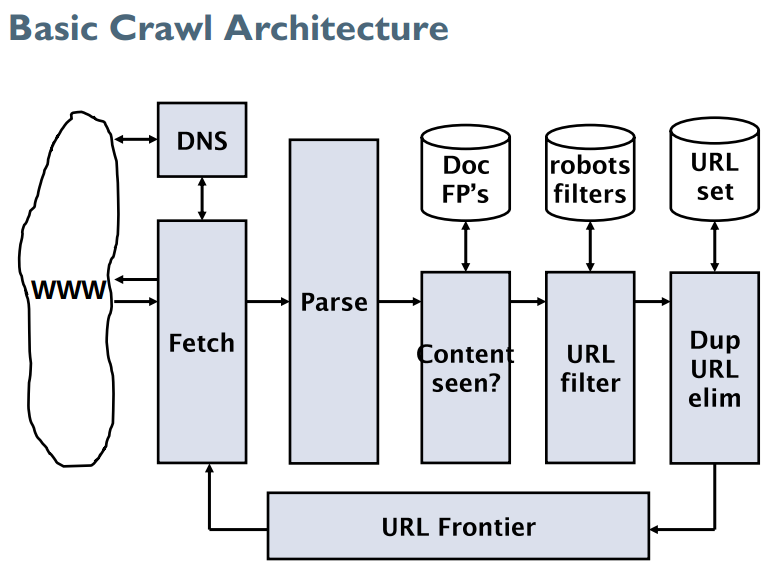
\includegraphics[width=0.7\linewidth]{./Media/basiccrawlarchitecture}
	\caption{Basic Crawl Architecture from Slides}
	\label{fig:basiccrawlarchitecture}
	\end{figure}
	
	It gets an url from the frontier, fetches the content if it can get past the `robots.txt' checker, parses out the word content and checks if that has already been seen, and adds it to the url filter after normalizing and checking if it does not already exist in the frontier or already visited urls.
	
	\subsection{Cut Corners}
	We could have used the Mercator scheme instead of just sleeping 1 second whenever the Crawler has finished with a page.
	
	The Crawler does find every url in the visited urls, but rather just the ones that are inside href attribute.
	
	The Crawler was limited to very few pages, 100-1000 primarily because the shingling with sketches is extremely slow for some reason.
	
	To actually check for content it might be a good idea to remove all the tags from the HTML content retrieved, but we do not do that.
	
	The sketches for each document is kept in memory, which only works because we crawl very few pages.
	
	\section{Indexer}
	The purpose of the indexer is to sort through the crawled documents, and create something that can be easily utilized by the search engine by saying which pages contain which terms along with the frequency.
	The indexer retrieves the items in the database.
	These items contain the Html, Url and Document Id for the site.
	The Html is the important part here. The Html has its html tags and attributes removed, and what remains are words and these are tokenized by splitting them. 
	These words are made into features, by stemming them using an English premade stemmer and by removing the English stopwords.
	Here it is important to note that the query gets the same treatment, in that its tokenized, stemmed and stopwords are removed.
	That feature is then added to the inverted index along with the id of the document.
	
	Adding to the inverted index works as such, it receives the term and the document id as mentioned, checks if the inverted index, which is a dictionary with a string key where the term is the key, and a posting list that contains a list of postings.
	
	If the inverted index does not already contained the term, it creates a list of postings, adds a posting with the document id, and adds that to inverted index using the term and a new posting list.
	
	If the inverted index does contain it, it checks if the document id already has a posting in that we might encounter the same word multiple times in the same document. It then sorts the postings.
	
	Otherwise it increments the frequency the term has been seen in the current document.
	
	This inverted index is kept in memory, which only works because only a small amount of sites are actually crawled.
	
	The general architecture of the indexer can be seen in the figure below.
	
	\begin{figure}[H]
	\centering
	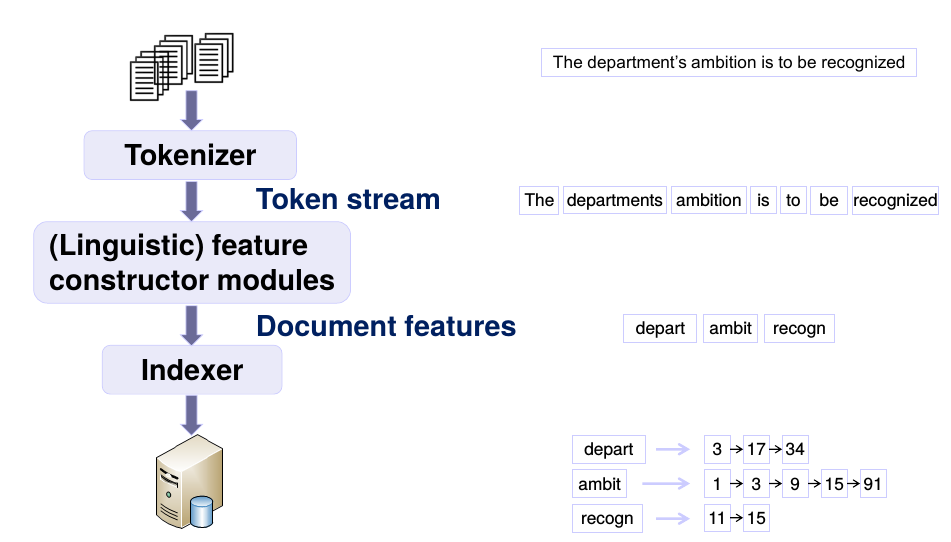
\includegraphics[width=0.7\linewidth]{./Media/indexer}
	\caption{}
	\label{fig:indexer}
	\end{figure}
	
	\section{Ranker}
	The purpose of the ranker is to get the most relevant results for the user given some query.
	For the ranker we used the cosine score algorithm based on tf-idf weighting.
	
	What the ranker does specifically is that it takes a query, tokenizes it and constructs features using the stemmer and stopword removal like in the indexer.
	
	The query weights are then constructed using the document frequency.
	
	These terms are then used to calculate a score for each document, and this is then used sort the results and provide a good output for the user, usually ~10 documents.
	
	\section{Demonstration}
	The query used was "internet of things"
	

\end{document}
